\section{Correlator Matrices}\label{sec:correlator_matrices}
In order to compute the low-lying finite-volume stationary states of QCD, we compute temporal correlator matrices of the form,
\begin{equation}
    \mathcal{C}_{i j}(t)=\bra 0 \mathcal O_{i}\left(t+t_{0}\right) \overline{\mathcal O}_{j}\left(t_{0}\right)\ket 0,
\end{equation}
where $\mathcal O_i(t+t_0)$ are the operators which annihilate the states of interest at a time $t+t_0$ and $\overline{\mathcal O}_j(t_0)$ are the corresponding operators which create the states of interest at an earlier time $t_0$. The operators are engineered such that the correlator matrix is Hermitian\footnote{This follows from the requirement that $\bra 0 O_i \ket n = \bra n \overline O_i \ket 0 ^*$.}. Since the energies are determined from the exponential decay rates of these two-point correlators, we can rescale the operators without changing the energy spectrum. In order to dampen the effects of differing normalizations among the operators, we rescale $\mathcal C(t)$ to form the actual correlator matrix $C(t)$ which we analyze as follows,
\begin{equation}
    C_{ij}(t) = \frac{\mathcal C_{ij}(t)}{\sqrt{\mathcal C_{ii}(\tau_N) \mathcal C_{jj}(\tau_N)}},
\end{equation}
where the \emph{normalization time} $\tau_N$ is taken at a very early time. Echoing the argument in Sec.~\ref{sec:intro_corr}, we can perform a spectral decomposition of $C(t)$ to obtain
\begin{equation}\label{eq:corr_spec_decomp}
    C_{i j}(t)=\sum_{n} Z_{i}^{(n)} Z_{j}^{(n) *} e^{-E_{n} t},
\end{equation}
where the $E_n < E_{n+1}$, the energies have been shifted such that $E_0\equiv 0$, and we have defined the \emph{overlap factors},
\begin{equation}
    Z_{j}^{(n) *}=\bra n \bar{O}_{j}\ket 0, \quad Z_{j}^{(n)}=\bra 0 O_{j} \ket n.
\end{equation}
The overlap factors offer us some insight into how much the state produced by a particular operator overlaps onto a particular energy eigenstate. This information can be used to make qualitative assessments of the contents of a particular energy state, e.g.\ if it is single- or multi-hadron dominated. Note that invariance under the a shift in phase
\begin{equation}
    Z_{j}^{(n)} \rightarrow Z_{j}^{(n)} e^{i \phi_{n}}
\end{equation}
implies that we can only determine the magnitude $|Z_j^{(n)}|$ of these overlap factors.
\section{The Generalized Eigenvalue Problem}
In the limit of infinite statistics, one could in principle fit Eq.~(\ref{eq:corr_spec_decomp}) and determine the entire energy spectrum. In practice, however, we are only able to fit the lowest one or two energies in the sum. It would be better to devise a method that allows us to fit more than just the lowest one or two energies in the spectrum. Ref.~\cite{Luscher:1990ck} proves a theorem that is the cornerstone for our approach to extracting energies from temporal correlators:
\begin{quote}
    \textbf{Theorem:} For every $t\geq 0$, 
    let $\lambda_n(t)$
    be the eigenvalues of an $N\times N$ Hermitian correlation matrix $C(t)$ ordered 
    such that
    $\lambda_0\geq \lambda_1\geq \dots\geq \lambda_{N-1}$, then 
    \begin{equation}
       \lim_{t\rightarrow\infty}\lambda_n(t)= b_n e^{-E_n t}\Bigl[1
     + \mathcal O(e^{-t\Delta_n})\Bigr],\qquad b_n>0,\quad
      \Delta_n = \min_{m\neq n}\vert E_n-E_m\vert.
    \label{eq:thmlarget}
    \end{equation}
\end{quote}
This tells us that a \emph{principal correlator} $\lambda_n(t)$ tends to a decaying exponential whose decay rate is the $n^{\rm{th}}$ energy of the spectrum. This theorem is still insufficient for use in practice, however. At large $t$ such that the $\mathcal O(e^{-t\Delta_n})$ correction is negligible, the determination of $C(t)$ has large uncertainties due to a decreasing signal-to-noise ratio~\cite{Lepage:1989hd}. At small $t$ such that $C(t)$ is well determined, the $\mathcal O(e^{-t\Delta_n})$ is not negligible. Fortunately, it is shown in Ref.~\cite{Luscher:1990ck} that the correction term can be brought down to $\mathcal O(e^{-t(E_N - E_n)})$ by instead solving the following generalized eigenvalue problem (GEVP):
\begin{equation}\label{eq:gevp}
    C(t) v_{n}\left(t, \tau_{0}\right)=\lambda_{n}\left(t, \tau_{0}\right) C\left(\tau_{0}\right) v_{n}\left(t, \tau_{0}\right), \quad n=1, \cdots, N-1, \quad \frac{t}{2} \leq \tau_0 < t.
\end{equation}
In practice, we find that a good rule of thumb to keep the $\mathcal O(e^{-t(E_N - E_n)})$ correction term low is to demand $N \geq \frac{3n}{2}$, where $n$ is the number of energies we wish to extract. Solving Eq.~(\ref{eq:gevp}) is equivalent to diagonalizing $G(t) = C^{-1 / 2}\left(\tau_{0}\right) C(t) C^{-1 / 2}\left(\tau_{0}\right)$, and the eigenvectors tend to~\cite{Blossier:2009kd}
\begin{equation}
    \lambda_{n}(t) \rightarrow\left|Z_{n}^{\prime}\right|^{2} e^{-E_{n} t}, \quad t \rightarrow \infty.
\end{equation}
The overlaps are determined by
\begin{equation}
    Z_{j}^{(n)} \approx C_{j k}\left(\tau_{0}\right)^{1 / 2} V_{k n}(t) Z_{n}^{\prime}\quad \text{(no sum over n)},
\end{equation}
where $V$ is the unitary matrix whose columns are the eigenvectors of $G(t)$.
\section{Pivots and Operator Pruning}\label{sec:pivots}
Two important assumptions about $C(t)$ are that it is Hermitian as well as positive-definite, which also implies that $G(t)$ is Hermitian and positive-definite. The assumption of positive-definiteness can be violated by operators that produce noisy correlators, or by an operator set that is linearly dependent. Noise can cause diagonal elements of the correlator to become zero or negative, and linearly dependent operators will produce eigenvalues of $C(t)$ that are zero. The odds of this occurring increases as we increase the number of operators in our correlator matrix. We call the process of judiciously choosing operators to ensure our correlator matrices remain well-conditioned \emph{pruning}. Pruning is necessary, but not sufficient for ensuring well-conditioned correlator matrices. It is still necessary to monitor for ill-conditioned matrices and take corrective action.

The condition number $\xi^{\rm{cn}}$ of a matrix is defined as the magnitude of the ratio of its maximum eigenvalue $\lambda_{\rm{max}}$ to its minimum eigenvalue $\lambda_{\rm{min}}$:
\begin{equation}
    \xi^{\rm{cn}} = \left|\frac{\lambda_{\rm{max}}}{\lambda_{\rm{min}}}\right|.
\end{equation}
When a matrix is ill-conditioned, its condition number will be high (and in some cases it may have negative eigenvalues). In order to prevent statistical noise from ruining our extraction of the energy spectrum, it is important to modify our diagonalization procedure to correct for high condition numbers, which is essentially introducing a singular value decomposition. These methods choose a threshold for the maximal allowed condition number $\xi^{\rm{cn}}_{\rm{threshold}}$ and project the correlator matrix onto the subspace spanned by the eigenvectors whose eigenvalues are larger than $\lambda_{\rm{threshold}} = \lambda_{\rm{max}}/\xi^{\rm{cn}}_{\rm{threshold}}.$ (The eigenvalues and condition numbers are all functions of $t$.)

Our entire method, which we call a pivot procedure, can be summarized as follows. Choose values for $\xi^{\rm{cn}(0)}_{\rm{max}}$, the maximal acceptable condition number for the $N\times N$ matrix $C(\tau_0)$. Let the $N_0 \leq N$ eigenvectors whose eigenvalues are greater than $\lambda^{(0)}_{\rm{max}}/\xi^{\rm{cn}(0)}_{\rm{max}}$ form the columns of the $N\times N_0$ matrix $P_0$, where $\lambda^{(0)}_{\rm{max}}$ is the largest magnitude of the eigenvalues of $C(\tau_0)$. Then define the $N_0\times N_0$ matrices
\begin{equation}
    \begin{aligned}
    \widetilde{C}\left(\tau_{0}\right)&=P_{0}^{\dagger} C\left(\tau_{0}\right) P_{0},\\
    \widetilde{C}(t)&=P_{0}^{\dagger} C(t) P_{0},\\
    \widetilde{G}(t)&=\widetilde{C}\left(\tau_{0}\right)^{-1 / 2} \widetilde{C}(t) \widetilde{C}\left(\tau_{0}\right)^{-1 / 2},
    \end{aligned}
\end{equation}
for $t\neq t_0$. We then solve for the eigenvectors and eigenvalues of $\widetilde G(t)$. Let the $N_P\leq N_0$ eigenvectors whose eigenvalues are greater than $\lambda^{(t)}/\xi^{(t))_{\rm{max}}}$ form the columns of the $N_0\times N_P$ matrix $\widetilde V(t)$, where $\lambda^{(t)}_{\rm{max}}$ is the largest magnitude of the eigenvalues of $\widetilde G(t)$. The $N_P\times N_P$ matrix
\begin{equation}
    \widetilde{\Lambda}(t)=\widetilde{V}^{\dagger}(t) \widetilde{G}(t) \tilde{V}(t)
\end{equation}
will satisfy
\begin{equation}
    \begin{aligned}
    &\widetilde{\Lambda}\left(\tau_{0}\right)=I,\\
    &\widetilde{\Lambda}(t)=\operatorname{diag}\left(\lambda_{n}(t)\right),
    \end{aligned}
\end{equation}
where $\lambda_n \rightarrow \left|\widetilde{Z}_{n}^{\prime}\right|^{2} e^{-E_{n} t}$ for large $t$ and $Z_{i}^{(n)} \approx P_{0 i j} \widetilde{C}_{j k}\left(\tau_{0}\right)^{1 / 2} \widetilde{V}_{k n}(t) \widetilde{Z}_{n}^{\prime}$. We can therefore fit the different $\lambda_n(t)$ for energies and overlap factors of the spectrum. The pivot method presented above involves rotating the correlator at every time slice, but in practice, this is not strictly necessary. We can instead take a simpler approach of diagonalizing $\widetilde G(t)$ at only one time $\tau_d$ chosen such that $\tau_d > \tau_0$, and using the same matrix to diagonalize at every other time, provided that the off-diagonal elements are statistically consistent with zero for all time slices $t \geq \tau_d$. Using the same transformation at every time slice is an ingredient in the \emph{single pivot} method, and is the procedure used in this work. Note that choosing $\tau_d \approx 2\tau_0$ ensures minimal contamination from higher lying states~\cite{Luscher:1990ck}.
\subsection{The Zero Temperature Assumption}
An important caveat to everything presented thus far is that we work in the assumption of a zero-temperature (i.e. infinite time extent) limit. Recall that the expression relating two-point correlators to a sum of decaying exponentials, given by Eq.~(\ref{eq:corr_decomp}) rests on the assumption that $t\ll T$, where $T$ is the time extent of the lattice. When calculating correlator matrix elements, this should be corrected to
\begin{equation}\label{eq:corr_thermal}
    \begin{aligned}
        \mathcal{C}_{i j} &=\left\langle\mathcal{O}_{i}(t) \overline{\mathcal{O}}_{j}(0)\right\rangle_{T} \\
        &=\frac{1}{Z_{T}} \operatorname{Tr}\left[e^{-H T} \mathcal{O}_{i}(t) \overline{\mathcal{O}}_{j}(0)\right] \\
        &=\frac{1}{Z_{T}} \sum_{n}\bra n e^{-H(T-t)} \mathcal{O}_{i}(0) e^{-H t} \overline{\mathcal{O}}_{j}(0)\ket n \\
        &=\frac{1}{Z_{T}} \sum_{n, m} e^{-E_{n}(T-t)} e^{-E_{m} t}\bra n \mathcal{O}_{i}(0)\ket m \bra m \overline{\mathcal{O}}_{j}(0)\ket n,
        \end{aligned}
\end{equation}
where
\begin{equation}
    \begin{aligned}
        Z_{T} & = \operatorname{Tr} e^{-H T} \\
        &=\sum_{n}\bra n e^{-H T}\ket n \\
        &=\sum_{n} e^{-E_{n} T}.
    \end{aligned}
\end{equation}
Only in the limit $T\rightarrow \infty$ does Eq.~(\ref{eq:corr_thermal}) agree with Eq.~(\ref{eq:corr_decomp}) and Eq.~(\ref{eq:corr_spec_decomp}). The thermal effects of finite time extent will manifest as backwards propagating modes which will be briefly discussed in Sec.~\ref{sec:fit_forms}. Fortunately, on the $32^3\times 256$ anisotropic lattice used in this work, these thermal effects (or temporal wrap-around effects) are negligible, and even on smaller lattices, we only find it necessary to account for backwards propagating modes for the lightest states.
\section{Fit Forms}\label{sec:fit_forms}
Fitting the diagonalized correlators is accomplished by forming fit ansatzes based on decaying exponentials, or symmetric exponentials when we wish to account for thermal effects. One such fit form is the single exponential,
\begin{equation}\label{eq:single_exp}
    C(t) = Ae^{-E t}.
\end{equation}
This form is strictly incorrect for finite $t$ due to excited state contamination (i.e.\ subleading exponential contributions from higher-lying states), but it is approximately correct for sufficiently large $t$. The single exponential has the advantage that it has few fit parameters and is thus less sensitive to statistical noise, but it has the disadvantage that it is highly sensitive to the minimum time used in the fit domain. The fit domain must only include times at which the subleading contributions are negligible.

We can account for the effects of higher-lying states by using a two-exponential fit,
\begin{equation}
    C(t)=A e^{-E t}\left(1+B e^{-\Delta^{2} t}\right),
\end{equation}
where the term $\Delta^2$ is used to ensure that the gap to the next energy is positive. We can also attempt to account for higher-lying states by using an ansatz that mocks up these states as a sum of equally-spaced levels above the fit energy $E$, which is a simple, approximate way to account for much excited state contamination with relatively few parameters:
\begin{equation}
    C(t)=\frac{A e^{-E t}}{1-B e^{-\Delta^{2} t}} = Ae^{-Et}\left(\sum_{n=0}^\infty B^n e^{-\Delta^{2}t}\right).
\end{equation}
These forms have the advantage that they are less sensitive to the fit domain and more accurately model the theory, but they have the disadvantage that they contain more parameters than the single exponential and are more sensitive to statistical noise. For this reason, we must often resort to using a single-exponential fit for noisier correlators.

If we wish to account for thermal effects for mesons, we can also make any fit form symmetric, e.g.\
\begin{equation}
    C(t)=A\left(e^{-E t}+e^{-E(T-t)}\right)
\end{equation}
for the single exponential fit form. For baryons, things become more complicated, since the backwards propagating mode actually corresponds to a baryon's parity partner, which would necessitate fitting in two symmetry channels simultaneously. Fortunately, baryons are heavy enough that accounting for temporal wrap-around effects is usually not necessary. Note that no extra parameters are needed for this, so it is easy to verify if such fit forms are necessary. Additionally, a constant can be added to any of the fit forms to help account for vacuum expectation values and to account for thermal effects on smaller lattices.
\subsection{The Effective Energy}\label{sec:eff_mass}
A very useful tool in fitting correlators is the so-called \emph{effective energy} or \emph{effective mass} which is given by
\begin{equation}
    E_{\rm{eff}}(t) = -\frac{d}{dt}\ln C(t),
\end{equation}
which can be discretized and estimated as
\begin{equation}
    -\frac{1}{\Delta t}\left(\ln C(t+\Delta t)-\ln C(t)\right).
\end{equation}
The effective energy is designed such that it tends to the fit energy $E$ as $t\rightarrow \infty$. When performing our fits, we are usually visually guided by effective energy plots rather than the correlators themselves, but it is crucial to emphasize that we do not fit the effective energy itself. An example of an effective energy plot is given in Fig.~(\ref{fig:eff_en_ex}).

\begin{figure}
    \centering
    \hspace*{-0.75in}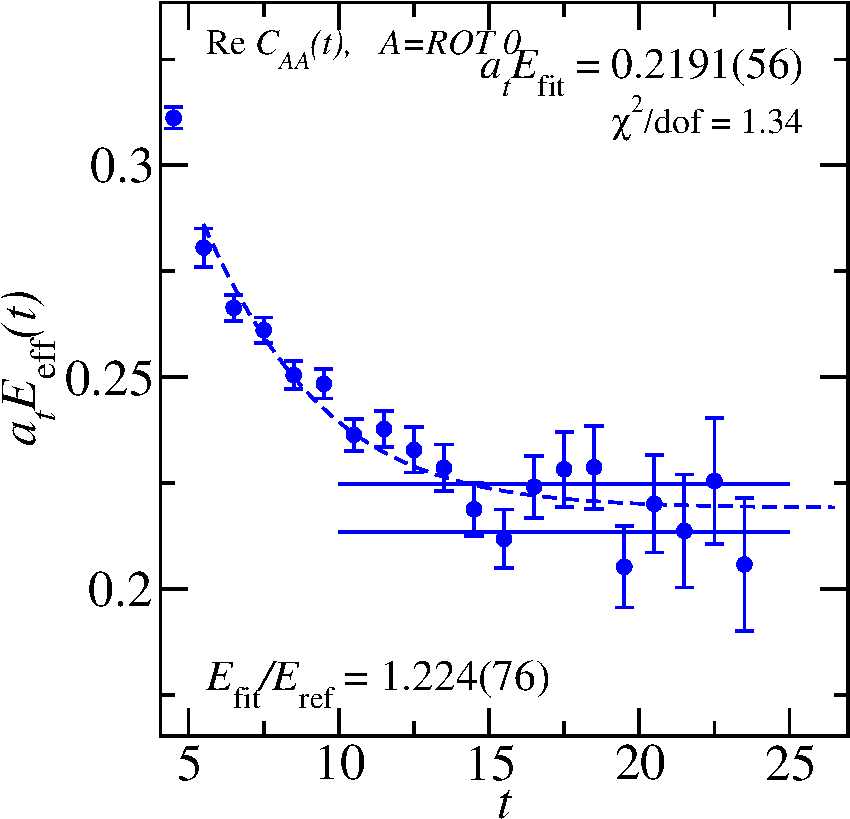
\includegraphics[width=0.6\textwidth]{figures/effmass.pdf}
    \caption[Example of an effective energy plot.]{Example of an effective energy plot. A curve obtained from a two-exponential correlator fit is overlaid, along with horizontal bars above and below the plateau, which depict the confidence interval of the energy of the leading exponential.}\label{fig:eff_en_ex}
\end{figure}

\section{Error Analysis and Resampling}
The observables we estimate through direct Monte Carlo measurements on gauge configurations are called \emph{simple} observables. Estimating the variance of simple observables is straightforward via calculating the population variance using the Monte Carlo method. All other observables are called \emph{non-simple} observables. An example of a non-simple observable is a model parameter obtained when we fit a correlator to data points which are themselves averages over many gauge configurations. The way to approach error analysis for non-simple observables is through \emph{resampling} techniques. Resampling involves forming new datasets from an initial dataset in order to estimate properties of how that dataset is distributed. For example, if we wanted to estimate the variance of the mean of some variable $x$, we would need several sets of measurements $\{x\}_i$ from which we can estimate the variance of the mean as
\begin{equation}
    \sigma^2_{\overline x} = \langle  \overline x^2 \rangle  - \langle \overline x \rangle ^2,
\end{equation}
where $\overline x$ denotes the population mean of a single set, and $\langle\rangle$ denotes the average over all populations $\{x\}_i$. In general, we wish to inquire about any arbitrary property of a set $\{x\}$. When only one dataset $\{x\}$ is available, resampling can be used to form new sets $\{x\}_i$ using only the original set. The dataset we consider is a set of gauge configurations $\{U\}$. Here we outline two resampling techniques, namely the \emph{jackknife} and the \emph{bootstrap}~\cite{efron1982jackknife}.

Jackknife resampling proceeds as follows. For a set of $N_c$ configurations $\{U\}$, form new sets $\{U\}_i$ which consist of every configuration in $\{U\}$ \emph{except} for the $i^{\rm{th}}$ configuration. There will be $N_c$ such new sets, and we expect that because only one configuration has been removed from each, that any properties we measure of the set will be close to those of the original set.

Bootstrap resampling proceeds as follows. For a set of $N_c$ configurations $\{U\}$, form $N_b$ new sets $\{U_i\}$ by choosing $N_c$ configurations from $\{U\}$ randomly with replacement. Since configurations can be sampled multiple times or not at all, we do not expect that properties we measure of the resampled sets will necessarily be distributed closely to that of the original set, as we do with jackknife resampling.

The properties we wish to estimate are the covariances of our model fit parameters, such as the energies and overlap factors. For jackknife resampling, we estimate the covariance as
\begin{equation}
    \operatorname{cov}(f_i, f_j) = \frac{N_c - 1}{N_c}\sum_{i=1}^{N_c}\left(\langle f \rangle_i - \langle f \rangle^J\right)\left(\langle f \rangle_j - \langle f \rangle^J\right),
\end{equation}
where $\langle f \rangle_i$ denotes the average of $f$ over the $i^{\rm{th}}$ jackknife resampling, and $\langle f \rangle^J$ denotes the average of $f$ over all resamplings. For bootstrap resampling, we estimate the covariance as
\begin{equation}
    \operatorname{cov}(f_i, f_j) = \frac{1}{N_b-1}\sum_{i=1}^{N_b}\left(\langle f \rangle_i - \langle f \rangle^B\right)\left(\langle f \rangle_j - \langle f \rangle^B\right),
\end{equation}
where $\langle f \rangle_i$ denotes the average of $f$ over the $i^{\rm{th}}$ bootstrap resampling, and $\langle f \rangle^B$ denotes the average of $\langle f \rangle_i$ over all bootstrap resamplings.
\section{Correlated $\chi^2$ Minimization}
For uncorrelated data, it is usually sufficient to fit the model parameters $\bs \alpha$ of a function $f(t;\bs \alpha)$ correlator data $C(t)$ by minimizing the uncorrelated $\chi^2$ metric defined by
\begin{equation}
    \chi^{2}=\sum_{t} \frac{(C(t)-f(t;\bs\alpha))^{2}}{\sigma_{t}^{2}},
\end{equation}
where $\sigma_t^2$ is the variance of the data at each time point. Our measurements are not statistically independent, however, because each measurement is taken on the same set of gauge configurations. We must therefore fit our correlators by instead minimizing the correlated $\chi^2$, defined by
\begin{equation}\label{eq:corr_chisq}
    \chi^{2}= \sum_{t,t^\prime} = \left(C(t) - f(t;\bs\alpha)\right)\operatorname{cov}^{-1}\left(C(t), C(t^\prime)\right)\left(C(t^\prime) - f(t^\prime; \bs\alpha)\right).
\end{equation}
The model parameters are then fit by minimizing $\chi^2$ on each resampling and calculating their uncertainties using the relevant covariance formula for the given resampling scheme.